\documentclass{article}
\usepackage[margin=1.1in]{geometry}
\usepackage[utf8]{inputenc}
\usepackage{graphicx}
\usepackage{booktabs}

%opening
\title{Scan chain based testing mechanism for digital systems }
\author{Advisor : Prof. Madhav P. Desai \\ \\Titto Thomas \\ Wadhwani Electronics Laboratory \\ EE Dept. IIT Bombay}

\begin{document}
\maketitle

\begin{abstract}
The document proposes a design for testing the hardware descriptions implemented on any general CPLD / FPGA board. It will be tested on Krypton board ( Developed by WEL Lab ) having Max V CPLD from \textit{Altera}, placed on a custom designed PCB board. The proposed design uses a scan chain based architecture similar to the industry testing standard, JTAG. With a standard set of additions to the hardware description of the Device Under Test (DUT), it's working could be tested for any set of inputs given. As the entire process can be controlled through a PC, it's relatively easier and faster than hardware testing.
\end{abstract}

%------------------------------------Intro-----------------------------------------------------
\section{Introduction}
The system is aimed to test the digital system design, i.e, send input combinations to the hardware and read back their outputs. The complete system has mainly three parts. The first one is a software running on the host PC that takes the command inputs from the user. Second one is a microcontroller board that converts the commands (passes through USB) into a set of signals for the Krypton board. The final one is the krypton board containing both the hardware description and the proposed additional tester design.

\begin{figure}[h!]
\centering
% XCircuit output "scan_main.tex" for LaTeX input from scan_main.ps
\def\putbox#1#2#3#4{\makebox[0in][l]{\makebox[#1][l]{}\raisebox{\baselineskip}[0in][0in]{\raisebox{#2}[0in][0in]{\scalebox{#3}{#4}}}}}
\def\rightbox#1{\makebox[0in][r]{#1}}
\def\centbox#1{\makebox[0in]{#1}}
\def\topbox#1{\raisebox{-0.60\baselineskip}[0in][0in]{#1}}
\def\midbox#1{\raisebox{-0.20\baselineskip}[0in][0in]{#1}}
   \scalebox{1}{
   \normalsize
   \parbox{6.75in}{
   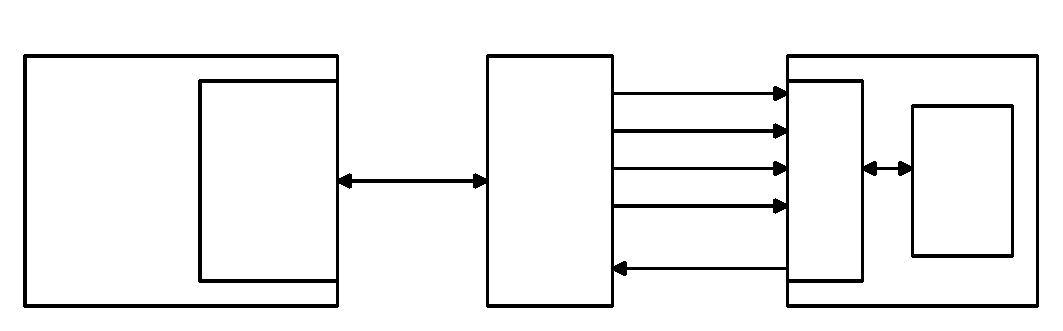
\includegraphics[scale=0.9]{scan_main.eps}\\
   % translate x=1040 y=64 scale 0.38
   \putbox{0.78in}{1.65in}{1.20}{PC}%
   \putbox{2.7in}{1.65in}{1.20}{ATxMega128}%
   \putbox{4.8in}{1.65in}{1.20}{DE0-Nano}%
   \putbox{1.23in}{0.9in}{1.20}{Python}%
   \putbox{1.28in}{0.7in}{1.20}{Script}%
   \putbox{2.02in}{0.6in}{1.20}{USB link}%
   \putbox{3.9in}{1.38in}{1.20}{{\small TDI}}%
   \putbox{3.87in}{1.15in}{1.20}{{\small TCLK}}%
   \putbox{3.9in}{0.92in}{1.20}{{\small TMS}}%
   \putbox{3.87in}{0.68in}{1.20}{{\small TRST}}%
   \putbox{3.9in}{0.11in}{1.20}{{\small TDO}}%
   \putbox{4.8in}{0.35in}{1.20}{\rotatebox{-270}{Scan Chain}}%
   \putbox{5.48in}{0.81in}{1.20}{DUT}%
   } % close 'parbox'
   } % close 'scalebox'
   \vspace{-\baselineskip} % this is not necessary, but looks better
\\
\end{figure}
The software side will be like a shell that repeatedly takes inputs from the user. There will be a standard set of commands to be used along with their parameters. The PC is connected to the microcontroller through a USB link , with a predefined standard data transfer scheme. 
The microcontroller will translate the commands, and generate corresponding signals through it's port pins. The hardware description of DUT and the tester hardware are bundled together and implemented on the Krypton board. Further design details and specifications are explained in the following sections.

%---------------------------------Software-----------------------------------------------------
\section{Software shell}
It will be a shell emulating script written in python. It gives a terminal like environment for the user to enter the commands for testing.
The back-end USB communication to the microcontroller is handled by a \texttt{pyUSB} python package. It contains functions to detect, connect and communicate to a specific device connected through USB. All the software commands in capital letters and will have some optional arguments.
\paragraph*{}
The inputs should be passed as a text file, with each row containing exactly one bit of the input. The output will also be written back into a specified output file. The commands to be entered along with their syntax are tabulated below.

\begin{center}

\begin{table}[h]
\begin{tabular}{@{}p{7cm}p{9cm}@{}}
\toprule
 \textbf{Command} &  \textbf{Details}\\ \toprule
 CONNECT &  Establish a connection to the Microcontroller board and display the status of the board.\\ \midrule
 PRELOAD $<in\; pins>$ $<in\; file>$ &  Load the inputs from $in\;file$ to the scan chain of the tester. The $in\; pins$ indicates the number of input pins the design has ( also the number of entries in the input file ).\\ \midrule
 SAMPLE $<out\; pins>$ $<out\; file>$ &  Read out the scan chain and store the output in $out\; file$. The $out\; pins$ indicates the number of output pins the design has.\\ \midrule
 DETACH &  Disconnect the microcontroller board and terminate communication.\\ \midrule
 QUIT &  Terminate the shell program.\\
 \bottomrule
\end{tabular}
\end{table}
 
\end{center}
%------------------------------ Microcontroller------------------------------------------------
\section{Microcontroller}
The microcontroller just does the conversion of text commands into their corresponding electrical signal sequences. It acts as a bridge between the user and the CPLD / FPGA board. This design propose to use the Ptx-128 board ( based on ATxMega128 ) developed in WEL Lab for this purpose.
\paragraph*{}
There are 5 signals communicating between the microcontroller and the Krypton board. They are
\begin{itemize}
 \item \texttt{TDI} : The serial test data input to be loaded in the scan chain.
 \item \texttt{TMS} : The commands for the TAP ( Test Access Port ) controller are passed serially through this pin.
 \item \texttt{TCLK} : The clock reference for all the other communication lines.
 \item \texttt{TRST} : Pin to reset the TAP controller at any instant.
 \item \texttt{TDO} : The serial data output from the scan chain.
\end{itemize}



%----------------------------- Tester design -------------------------------------------------------------------------------------------
\section{Tester Design}
The Tester design will have mainly 3 parts, one controller and two sets of registers. The first part will be a TAP controller, that takes the inputs from \texttt{TMS} at the rising edge of \texttt{TCLK} and sends out signals for the other parts after considering it's current state. The second part will be a Data Register (DR) which can be more than one in number ( the boundary scan chain being one among them ) that stores the input / output values. Third one is an Instruction Register (IR) which contains the number of DR being activated, the operation being executed etc.. These registers can be programmed by passing appropriate values through \texttt{TDI} and applying signals through \texttt{TMS}
\paragraph*{}
In this proposed implementation, there will be only one DR ( the boundary scan chain ) and no IR.

\subsection{Modified latch design}
The boundary scan registers would contain a special type of latches. They have basically 3 operations Capture, Shift and Update. The design is shown below.

\begin{figure}[h!]
\centering
\input{latch.tex}\\
\end{figure}

If the test mode is not enabled, this latch will be bypassed ( Parallel In directly connected to Parallel Out ) and the data will not be stored. And if it is in test mode, then the latches will be added to the path. First operation will be to \textit{capture}, where the first latch would store the parallel input bit ( Storing output after computation ). The second one is an optional \textit{shift}, which would enable scanning in and out of the bits through a serial path. The final one is \textit{update}, when the output of the first latch is copied on to the second ( Applying the input sequence to the circuit ).

\subsection{Overall hardware design}
The complete hardware on the CPLD / FPGA board will have a structure shown below. The tester hardware would contain the TAP controller, DR and IR registers. 
But, in the current implementation there is no IR, and the boundary scan register itself is the only DR. \texttt{DR\_REG} \& \texttt{IR\_REG} are a set of signals used to enable (\texttt{DR\_EN}, \texttt{IR\_EN}), clock (\texttt{DR\_CLK}, \texttt{IR\_CLK}) and reset (\texttt{DR\_RST}, \texttt{IR\_RST}) the corresponding register set.
\begin{figure}[h!]
\centering
\input{design.tex}\\
\caption{Tester hardware structure}
\end{figure}


\paragraph*{}
If the IR and multiple DR's were present, the \texttt{TDI} and \texttt{TDO} pins will be connected to either one of the DR's or bypassed all of them ( by passing through a single latch ) as decided by the IR.

\paragraph*{}
Now the TAP controller will control both the IR and DR, according to the input received through  \texttt{TMS}. It works according the FSM given below in the figure.
\begin{figure}[h!]
\centering
\input{flow.tex}\\
\caption{TAP controller state diagram}
\end{figure}
\end{document}
